% !TeX spellcheck = en_US
\chapter{Deep Learning for CV}
\todo{}

\section{Loss Functions}
L1-L2 loss doesn't work well with different \ac{CV} problems \cite{wang2009mean}. This section proposes some alternatives

\subsection{SSIM}
\ac{SSIM} measures the similarity between two images. \cite{wang2004image}
\begin{itemize}
	\item The \ac{SSIM} index is calculated on various windows of an image.
	\item Formula: Given two windows $x, y \in \mathbb{R}^{N \times N}$ (check \href{https://en.wikipedia.org/wiki/Structural_similarity}{Wikipedia})
	\begin{align}
		\text{SSIM}(x,y) &= \frac{(2\mu_x \mu_y + c_1) (2\sigma_{xy} + c_2)}{(\mu_x^2 + \mu_y^2 + c_1) (\sigma_x^2 + \sigma_y^2 + c_2)}\\
		\text{SSIM}(x,y) &= luminance(x,y) \cdot contrast(x,y) \cdot structure(x,y)
	\end{align}
	\item It is used in super-resolution problem.
\end{itemize}

\subsection{Perceptual Loss}
\label{subsec:perceptual-loss}
\begin{itemize}
	\item Perceptual Loss, \ac{aka} content loss or VGG loss, is the loss between the feature maps of two images, after passing through a few pretrained \ac{CNN} layers (\figref{fig:vgg-loss}).
	\item This loss is used in super-resolution problem
\end{itemize}

\begin{figure}[hbt!]
	\centering
	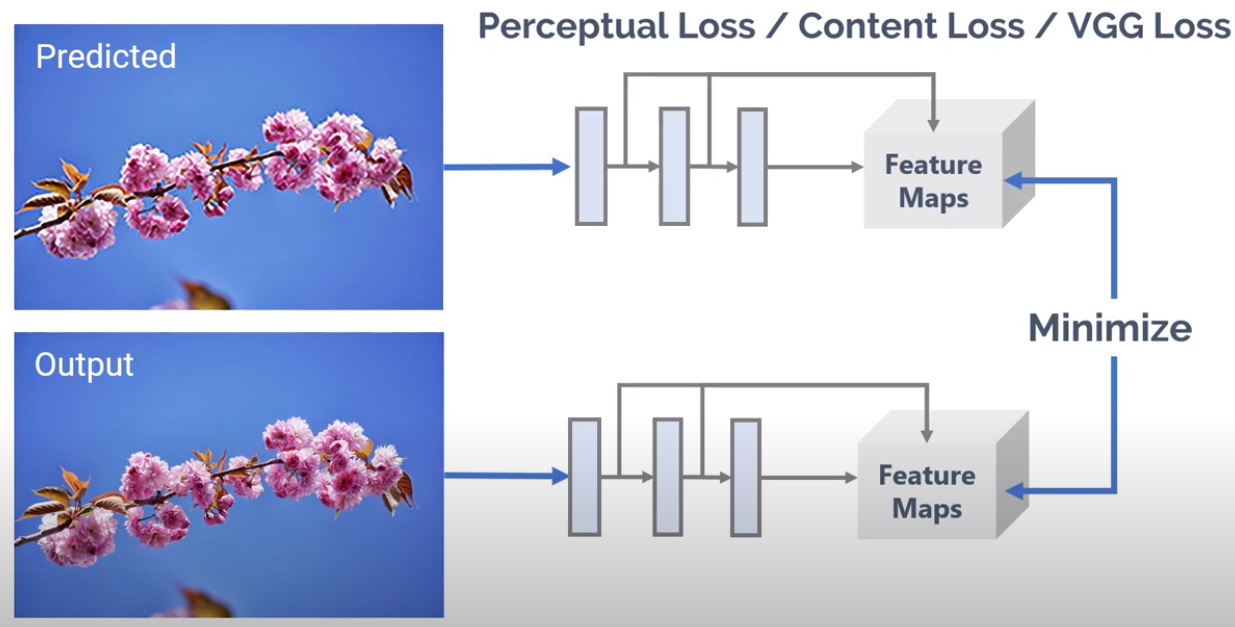
\includegraphics[width=0.7\textwidth]{vgg-loss.png}
	\caption{Perceptual loss is the loss between the feature maps, which are from passing images through a few frozen \ac{CNN} layers from VGG network.}
	\label{fig:vgg-loss}
\end{figure}

\subsection{FID}
In \ac{CV}, \ac{FID} is used to measure the distance between two distributions of two datasets, which are usually the original and the generated image datasets. \cite{heusel2017gans}
\begin{itemize}
	\item Pass the images through the pretrained Inception network, take the output right before the last layer.
	\item Calculate the mean and covariance matrices: $(\textbf{\textit{m}}, \textbf{\textit{C}})$ and $(\textbf{\textit{m}}_w, \textbf{\textit{C}}_w)$
	\begin{equation}
		d^2((\textbf{\textit{m}}, \textbf{\textit{C}}), (\textbf{\textit{m}}_w, \textbf{\textit{C}}_w)) = ||\textbf{\textit{m}} - \textit{\textbf{m}}_w||_2^2 + \text{Tr}(\textbf{\textit{C}} + \textbf{\textit{C}}_w - 2(\textbf{\textit{CC}}_w)^{1/2})
	\end{equation}
	\item The smaller the \ac{FID} value the better the generated images, obviously.
\end{itemize}

\subsection{PPL}
The high-level idea is such, when interpolation in the latent space may lead to non-linear changes in the image. 
\ac{PPL} is a metric to measure  the perceptually-based pairwise image distance. \cite{karras2019style}

\begin{align}
	l_{\mathcal{Z}} &= \mathbb{E} \left[ \frac{1}{\epsilon^2} d\left(G(\text{slerp}(\textbf{z}_1, \textbf{z}_2; t)), G(\text{slerp}(\textbf{z}_1, \textbf{z}_2; t + \epsilon))\right) \right] && \text{average in $\mathcal{Z}$ space}\\
	l_{\mathcal{W}} &= \mathbb{E} \left[ \frac{1}{\epsilon^2} d\left(g(\text{lerp}(f(\textbf{z}_1), f(\textbf{z}_2); t)), g(\text{lerp}(f(\textbf{z}_1), f(\textbf{z}_2); t + \epsilon))\right) \right] && \text{average in $\mathcal{W}$ space}
\end{align}

\begin{itemize}
	\item Latent vectors $\textbf{z}_1, \textbf{z}_2 \sim P(\textbf{z})$
	\item Interpolation functions: slerp and lerp.\\
	Basically, they also output a latent vector that lie on the interpolation path from $\textbf{z}_1$ to $\textbf{z}_2$
	\[\textbf{z}_t = \text{slerp}(\textbf{z}_1, \textbf{z}_2; t) \quad \text{with} \ t \sim U(0,1)\]
	\item $G$ is the generator, $g$ is the synthesis network, $f$ is the mapping network, thus $G = g \circ f$ and $image = G(\textbf{z})$ (\figref{fig:stylegan-generator})
	\item $d$ evaluates the perceptual loss given two generated images (\subsecref{subsec:perceptual-loss})
\end{itemize}

\section{Image-to-Image Translation}
Image-to-image translation is a class of computer vision problems where the goal is to learn the mapping between an input image and an output image. Recent approaches utilize \ac{GAN}. It has various applications \cite{isola2017image, zhu2017unpaired}, \eg:
\begin{itemize}
	\item Domain adaptation
	\item Semantic label $\leftrightarrow$ photo
	\item Map $\leftrightarrow$ aerial photo
	\item Edges $\rightarrow$ photo
	\item BW $\rightarrow$ color photos
	\item Day $\rightarrow$ night
	\item Photo with missing pixels $\rightarrow$ inpainted photo (recovering)
\end{itemize}

\subsection{pix2pix}
\texttt{pix2pix} uses \ac{CGAN} idea with U-Net architecture \cite{isola2017image}.
\begin{figure}[hbt!]
	\centering
	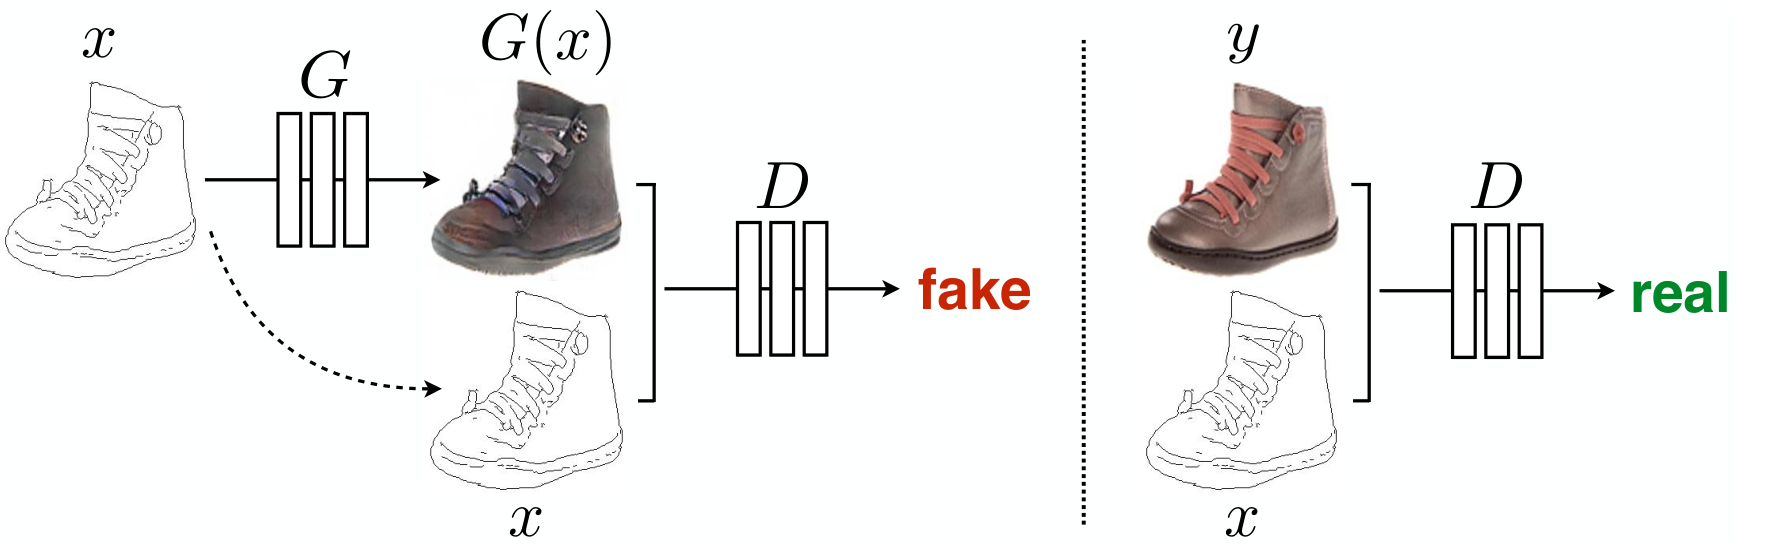
\includegraphics[width=0.9\textwidth]{pix2pix.png}
	\caption{Training a \ac{CGAN} to map edges $\rightarrow$ photo. Both the discriminator and generator are conditioned on the input $x$. \cite{isola2017image}}
\end{figure}

The loss function of \texttt{pix2pix} combines \ac{CGAN} objective with L1 distance with ground-truth images. L1 distance is prefer over L2 because L1 encourages less blurring effect.
\begin{align}
	\mathcal{L}_{GAN}(G,D) &= \mathbb{E}_y [\log D(y)] + \mathbb{E}_z [\log (1-D(G(z)))]\\
	\mathcal{L}_{CGAN}(G,D) &= \mathbb{E}_{x,y} [\log D(x,y)] + \mathbb{E}_{x,z} [\log (1-D(x,G(x,z)))]\\
	\mathcal{L}_{L1}(G) &= \mathbb{E}_{x,y,z} \big[ ||y-G(x,z)||_1 \big]\\
	G* &= \arg \underset{G}{\min} \underset{D}{\max} \mathcal{L}_{CGAN}(G,D) + \lambda \mathcal{L}_{L1}(G)
\end{align}

\note In implementation, the noise $z$ is accounted as DropOut percentage.

\subsection{CycleGAN}
Cycle\ac{GAN} addresses the problem when there is no \hlb{available paired training data}. By considering cycle consistency losses, it limits the mapping functions. \cite{zhu2017unpaired}
\begin{align}
	&G: X \rightarrow Y &&-\text{mapping from domain $X$ to domain $Y$}\\
	&F: Y \rightarrow X &&-\text{mapping from domain $Y$ to domain $X$}\\
	&F(G(x)) \approx x &&-\text{forward cycle consistency}\\
	&G(F(y)) \approx y &&-\text{backward cycle consistency}
\end{align}
\begin{align}
	\mathcal{L}_{GAN_1} (G, D_Y, X, Y) &= \mathbb{E}_{y \sim p_{data}(y)}[\log D_Y(y)] + \mathbb{E}_{x \sim p_{data}(x)} [\log (1 - D_Y(G(x)))]\\
	\mathcal{L}_{GAN_2} (F, D_X, X, Y) &= \mathbb{E}_{x \sim p_{data}(x)}[\log D_X(x)] + \mathbb{E}_{y \sim p_{data}(y)} [\log (1 - D_X(F(y)))]\\
	\mathcal{L}_{cyc}(G,F) &= \mathbb{E}_{x \sim p_{data}(x)}\big[||F(G(x))-x||_1 \big] + \mathbb{E}_{y \sim p_{data}(y)} \big[||G(F(y))-y||_1\big]\\
	\mathcal{L}(G, F, D_X, D_Y) &= \mathcal{L}_{GAN_1} (G, D_Y, X, Y) + \mathcal{L}_{GAN_2} (F, D_X, X, Y) + \lambda \mathcal{L}_{cyc}(G,F)\\
	G^*, F^* &= \arg\underset{G, F}{\min}\underset{D_X, D_Y}{\max} \mathcal{L}(G, F, D_X, D_Y)
\end{align}
\begin{figure}[hbt!]
	\centering
	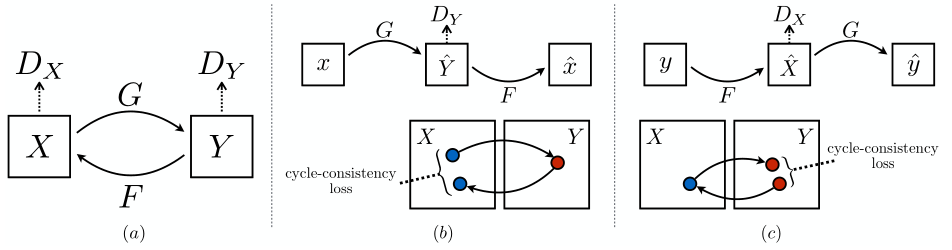
\includegraphics[width=\textwidth]{cyclegan.png}
	\caption{Cycle\ac{GAN} structure with 4 networks. \cite{zhu2017unpaired}}
\end{figure}

\note
\begin{itemize}
	\item The authors mention that experiment the cycle consistency loss as adversarial loss leads to no improved performance.
	\item Cycle\ac{GAN}'s results are not significantly better than pix2pix's.
	\item Perform well on tasks relating color transformation (\eg style transfer: picture $\leftrightarrow$ paintings, horse $\leftrightarrow$ zebra, winter $\leftrightarrow$ summer), but not so good with \hlb{geometric changes} (dog $\leftrightarrow$ cat).
\end{itemize}

\section{Neural Style Transfer}
Style transfer is similar to image-to-image translation, but doesn't require a dataset from each style. It instead runs an iterative optimization procedure on two given images.

\subsection{Artistic Style Transfer}
The first work is by \citeaus{gatys2015neural}. The authors manage to separate image content and image style. Given a \ac{CNN}, at the $l^{th}$ layer, there is $N_l$ distinct filters, thus, leads to $N_l$ feature maps of size $M_l$.
\begin{itemize}
	\item The image content is represented in matrix $F^l \in \mathcal{R}^{N_l \times M_l}$, which is the concatenation of these feature maps. $F^l_{ij}$ is the activation of the $i^{th}$ filter at position $j$ in $l^{th}$ layer. The authors prove this by trying to reconstruct the image from these feature maps.
	\begin{align}
		&\vec{p} &&-\text{original image}\\
		&\vec{x} &&-\text{generated image}\\
		&F^l_{ij} &&-\text{the original image's content }\\
		&P^l_{ij} &&-\text{the generated image's content}\\
		&\mathcal{L}_{content}(\vec{p}, \vec{x}, l) = \frac{1}{2} \sum_{i,j} \left( F^l_{ij} - P^l_{ij} \right) ^2 &&-\text{the content loss}
	\end{align}
	\item The image style is represented in the Gram matrix $G^l \in \mathcal{R}^{N_l \times N_l}$, where $G_{ij}^l$ is the correlation between feature map in the $l^{th}$ layer:
	\begin{equation}
		G_{ij}^l = \sum_k F_{ik}^l F_{jk}^l
	\end{equation}
	\begin{align}
		&\vec{a} &&-\text{artwork}\\
		&\vec{x} &&-\text{generated image}\\
		&A^l &&-\text{the artwork's style representation}\\
		&G^l &&-\text{the generated image's style representation}\\
		&E_l = \frac{1}{4 N^2_l M^2_l} \sum_{i,j} \left( G_{ij}^l - A_{ij}^l \right)^2 &&-\text{style representation loss at $l^{th}$ layer}	\\
		&\mathcal{L}_{style}(\vec{a}, \vec{x}) = \sum_{l=0}^L w_l E_l &&-\text{the style loss}
	\end{align}
\end{itemize}
\begin{align}
	&\mathcal{L}_{total}(\vec{p}, \vec{a}, \vec{x}) =  \alpha \mathcal{L}_{content}(\vec{p}, \vec{x})+ \beta \mathcal{L}_{style}(\vec{a}, \vec{x}) &&-\text{total loss}
\end{align}

The algorithm applies gradient descent to minimize the above loss with $\vec{x}$ as a white noise image in the beginning.

\subsection{Artistic Style Transfer for Videos}
Applying the above approach to video leads to terribly inconsistent results. \citeaus{ruder2016artistic} improve by adding additional improvements:
\begin{itemize}
	\item Short-term consistency by initialization: Estimate the optical flow between image $p^{(i)}$ and $p^{(i+1)}$. The generated image $x^{(i+1)}$ will not be initialized with a white noise image, but a warped image from the previous one: $x'^{(i+1)} = \omega_i^{i+1} (x^{(i)})$. Here $\omega_i^{i+1}$ denotes the warping function using the estimated optical flow.
	\item Temporal consistency loss
	\item Long-term consistency
	\item Multi-pass algorithm
\end{itemize}

\subsection{Fast Artistic Style Transfer}
The above style transfer approaches require an iterative optimization process for each pair of images. \citeaus{johnson2016perceptual} propose a training pipeline to simplify this procedure. By learning a network that minimize the same loss, the output now requires only one single run.
\begin{figure}[hbt!]
	\centering
	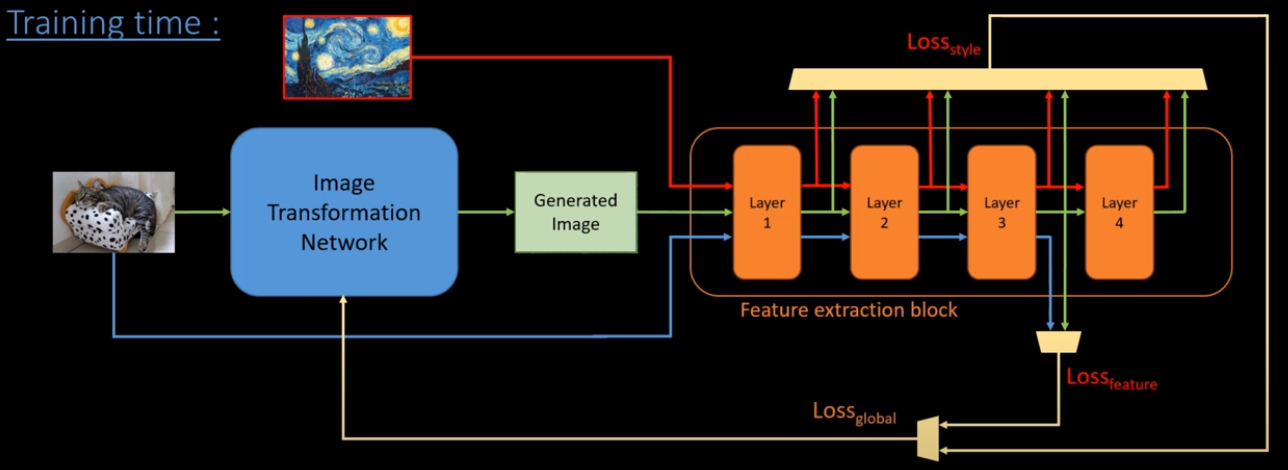
\includegraphics[width=\textwidth]{fast-artistic-style-transfer.png}
	\caption{Training pipeline (\href{https://youtu.be/VQEMptfWpLk}{src}) \cite{johnson2016perceptual}}
\end{figure}

\[\begin{matrix*}[l]
	\color{Green} + \text{Running in real-time}\\
	\color{red} - \text{Loss some temporal consistency when applying to videos}\\
	\color{red} - \text{One single style for a network}
\end{matrix*}\]

\subsection{Arbitrary Style-Transfer in Real-time}
\citeaus{huang2017arbitrary} improves prior methods::
\begin{itemize}
	\item Using \ac{AdaIN}
	\item Pros: $\begin{matrix*}[l]
		\color{Green} + \text{Running in real-time}\\
		\color{Green} + \text{A single network capable of transfer multiple arbitrary styles}
	\end{matrix*}$
\end{itemize}

Check their \href{https://youtu.be/IIRxJvW6bE4}{CVF presentation video}.

\section{Super Resolution}
Super Resolution is a \ac{CV} problem, in which we want to upscale a lower resolution image to a higher resolution one.
\begin{itemize}
	\item \href{https://youtu.be/KULkSwLk62I}{Youtube: How Super Resolution Works}
	\item Naive approach: nearest neighbor would simply spread the pixels out, then fill in the gap by copying values.
	\item Taking average, median would lead to better result, which is what bilinear and bicubic interpolation do.
\end{itemize}

\subsection{SRCNN}
\citeausm{dong2015image}'s model is a \ac{CNN} that (\figref{fig:SRCNN})
\begin{itemize}
	\item takes in a lower resolution image and output a higher resolution image
	\item the loss is simply squared error between the output with ground truth image
\end{itemize}

\begin{figure}[hbt!]
	\centering
	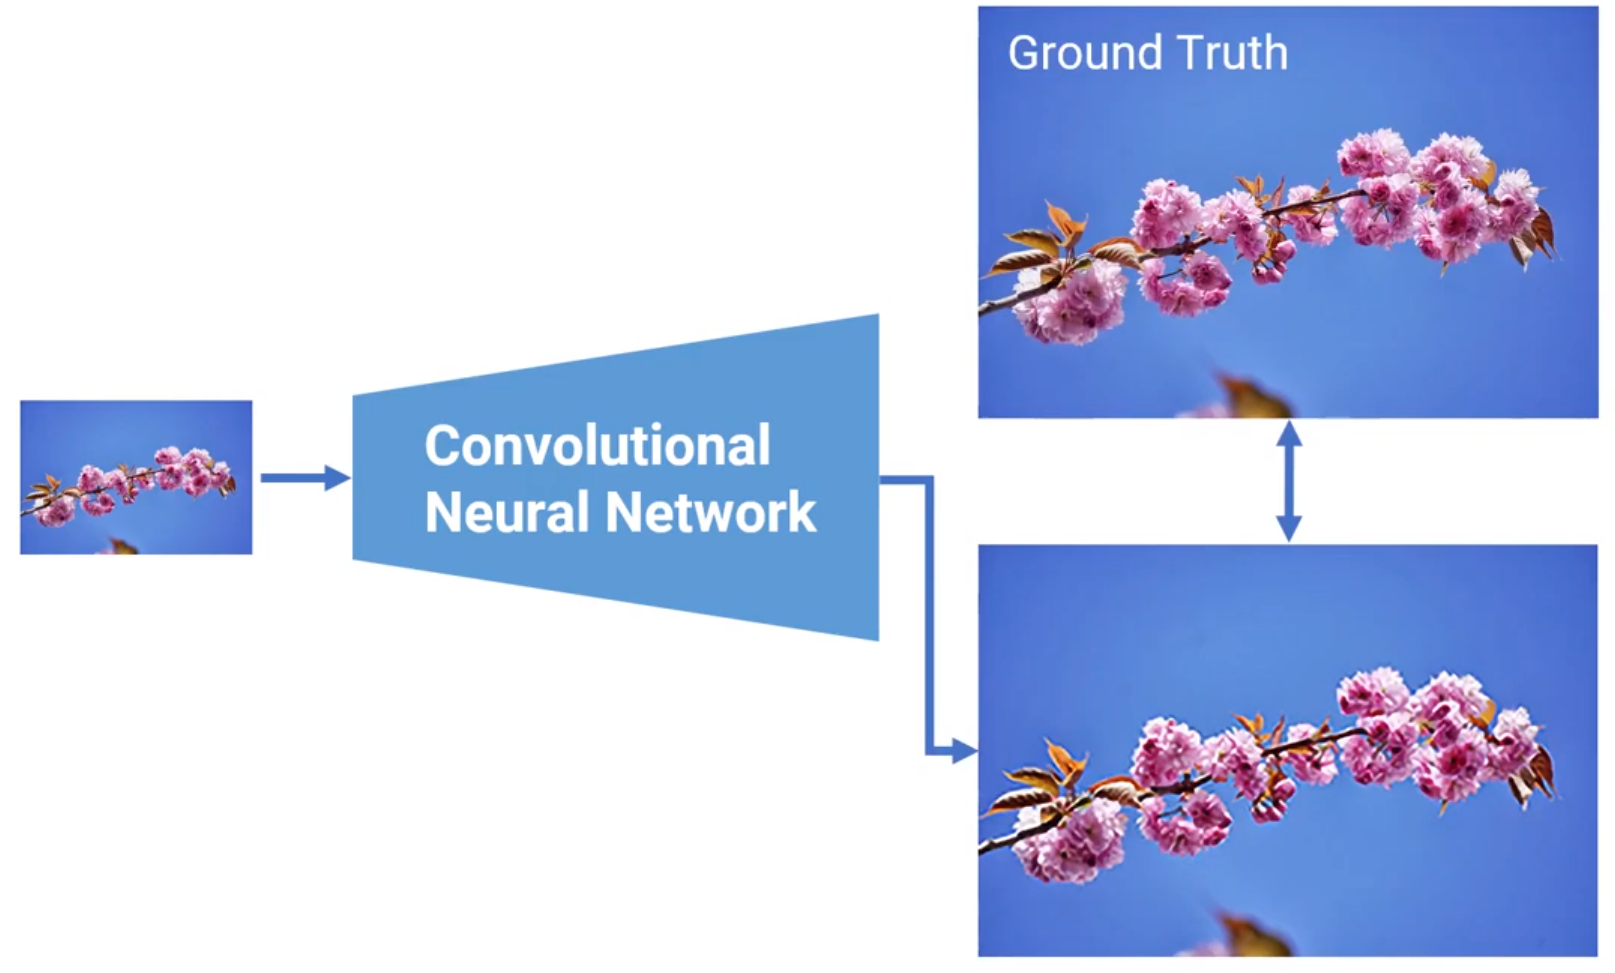
\includegraphics[width=0.7\textwidth]{SRCNN.png}
	\caption{\ac{SRCNN} training \cite{dong2015image}}
	\label{fig:SRCNN}
\end{figure}

\subsection{SRGAN}
\citeausm{ledig2017photo} use \ac{GAN}'s framework (\figref{fig:SRGAN}). The authors use VGG-based loss function

\begin{figure}[hbt!]
	\centering
	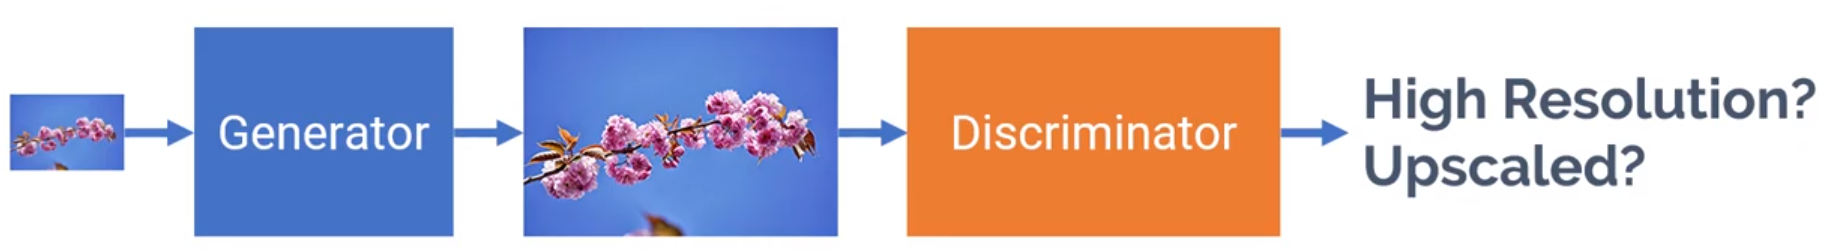
\includegraphics[width=\textwidth]{SRGAN.png}
	\caption{\ac{SRGAN} training \cite{ledig2017photo}}
	\label{fig:SRGAN}
\end{figure}

\subsection{ESRGAN}
\ac{ESRGAN} \cite{wang2018esrgan}
\begin{itemize}
	\item Remove \ac{BatchNorm}
	\item More layers and connections: residual scaling
	\item Modify the VGG loss: compare the feature maps before activation layers.
	\item Relativistic discriminator
\end{itemize}

\subsection{Further Improvements}
\begin{itemize}
	\item Network interpolation \cite{wang2018esrgan, wang2019deep}
	\item Contextual bilateral loss \cite{zhang2019zoom}
	\item Real-\ac{ESRGAN} \cite{wang2021realesrgan}
\end{itemize}

\subsection{Codes}
\begin{itemize}
	\item \href{https://github.com/xinntao/ESRGAN}{\ac{ESRGAN}} \cite{wang2018esrgan}
	\item \href{https://github.com/xinntao/Real-ESRGAN}{Real-\ac{ESRGAN}} \cite{wang2021realesrgan}
\end{itemize}

\section{StyleGAN}
\subsection{Initial Work}
\begin{itemize}
	\item Watch \href{https://youtu.be/kSLJriaOumA}{Tero Karras FI Youtube video}
	\item StyleGAN is image generation with style control. \cite{karras2019style}
	\item Key points on StyleGAN.v1's structure (\figref{fig:stylegan-generator}):
	\begin{itemize}
		\item Add mapping and styles via mapping network $f$ and \ac{AdaIN}
		\item Replace traditional input with a learnable constant \texttt{$4 \times 4 \times 512$}
		\item Add noise inputs at different levels: coarse ($4^2-32^2$) to fine layers ($64^2-1024^2$) with different scaling $B$
		\item Mixing regularization: use different style inputs from different latent vectors at different levels
	\end{itemize}
\end{itemize}

\subsection{Slider stuff}
With some additional steps, one could create a slider to gradually change different attributes, \eg gender, hair styles (\href{https://youtu.be/dCKbRCUyop8}{Arxiv Insights}).

\subsection{Truncation Trick}
Drawing latent vectors from a truncated sampling space tends to improve average image quality, with some loss in variation:
\begin{itemize}
	\item Compute center of mass of $\mathcal{W}$: $\bar{\textbf{w}} = \mathbb{E}_{\textbf{z} \sim P(\textbf{z})}[f(\textbf{z})]$
	\item Given a vector $\textbf{w}$, scale it: $\textbf{w}' = \bar{\textbf{w}} + \psi(\textbf{w} - \bar{\textbf{w}})$, where $|\psi| < 1$
	\item Varying $\psi$ value also gives us the nice interpolation effect (\figref{fig:stylegan-truncation})
	\begin{figure}[hbt!]
		\centering
		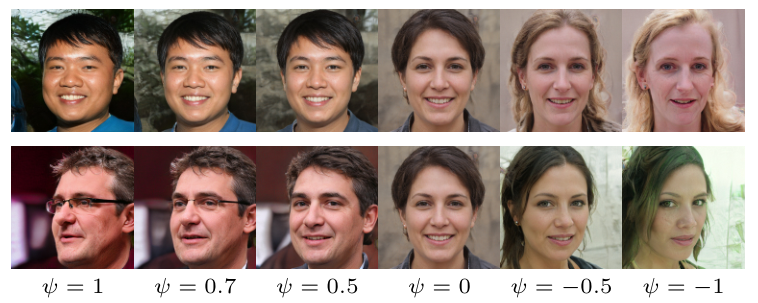
\includegraphics[width=0.7\textwidth]{stylegan-truncation.png}
		\caption{Effect of truncation trick}
		\label{fig:stylegan-truncation}
	\end{figure}
\end{itemize}

\subsection{Improvements}
Improvements to StyleGAN.v1 to handle droplet and phase artifacts:
\begin{itemize}
	\item \href{https://youtu.be/c-NJtV9Jvp0}{StyleGANv2} \cite{karras2020analyzing}
	\begin{itemize}
		\item Replacing \ac{AdaIN} with \ac{CNN} weight demodulation and moving addition of noise outside of style area (\figref{fig:stylegan-weight-demodulation})
		\begin{align}
			w'_{ijk} &= s_i \cdot w_{ijk}\\
			w''_{ijk} &= \frac{w'_{ijk}}{\sqrt{\sum_{i,k} {w'_{ijk}}^2 + \epsilon}}
		\end{align}
		\begin{figure}[hbt!]
			\centering
			\begin{subfigure}[b]{0.55\textwidth}
				\centering
				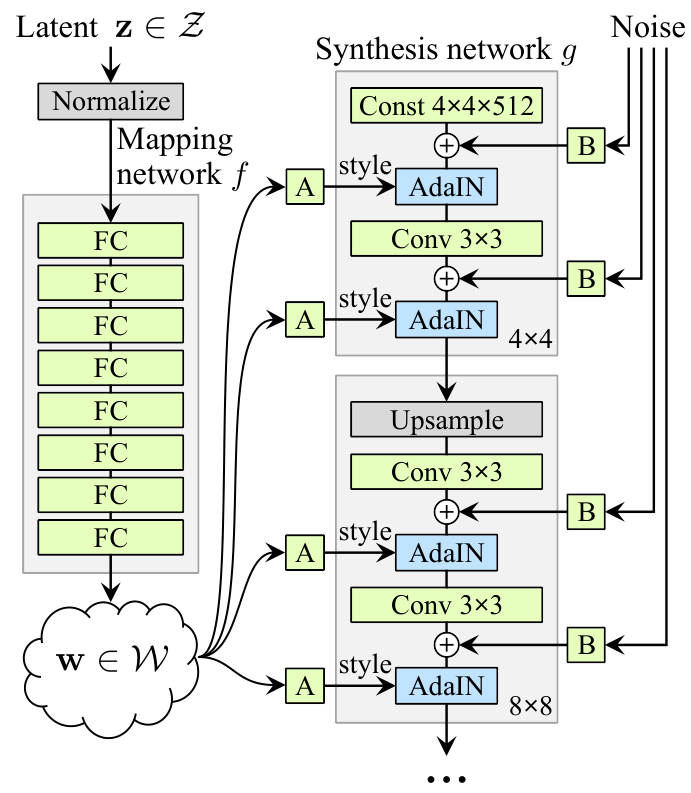
\includegraphics[width=\textwidth]{stylegan-generator.png}
				\caption{StyleGANv1's structure \cite{karras2019style}.}
				\label{fig:stylegan-generator}
			\end{subfigure}
			\hfill
			\begin{subfigure}[b]{0.4\textwidth}
				\centering
				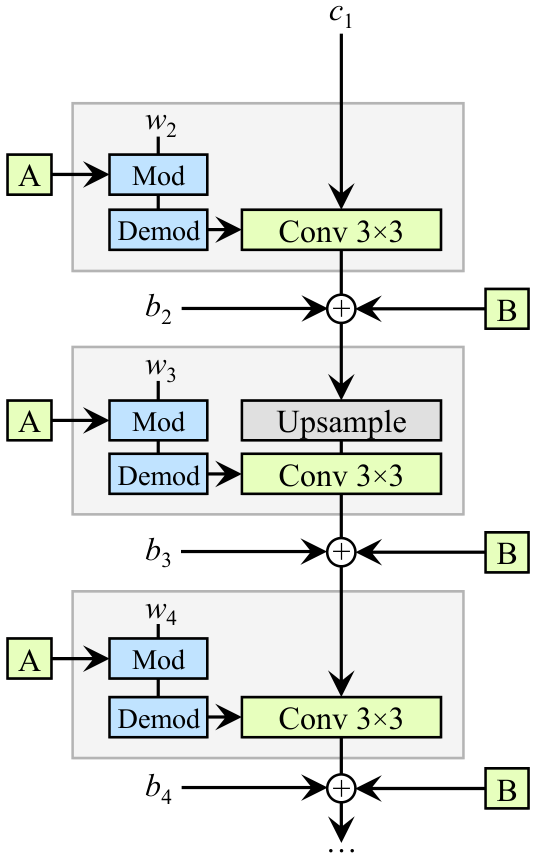
\includegraphics[width=\textwidth]{stylegan-weight-demodulation.png}
				\caption{Weight demodulation \cite{karras2020analyzing}.}
				\label{fig:stylegan-weight-demodulation}
			\end{subfigure}
			\caption{StyleGAN architectures.}
			\label{fig:stylegan}
		\end{figure}
		\item Lazy regularizer with \ac{PPL}
		\item Replacing progressive growing with skip connections and residual modules.
		\item Finally, it trains faster
	\end{itemize}
	\item StyleGAN3 suggests even more changes to deal with sticking texture artifacts (check \href{https://youtu.be/j1ZY7LInN9g}{bycloud} and \href{https://youtu.be/_euFoyLEyqU}{Andrew Melnik} videos) \cite{karras2021alias}
\end{itemize}

\section{Code Examples}
\begin{itemize}
	\item \href{https://www.tensorflow.org/tutorials/generative/pix2pix}{\texttt{Tensorflow}'s tutorial: pix2pix}
	\item \href{https://www.tensorflow.org/tutorials/generative/cyclegan}{\texttt{Tensorflow}'s tutorial: CycleGAN}
	\item \href{https://github.com/manuelruder/artistic-videos}{\texttt{Github} source code: Artistic Style Transfer for Videos}
	\item \href{https://www.tensorflow.org/tutorials/generative/style_transfer}{\texttt{Tensorflow}'s tutorial: Neural style transfer}
	\item \href{https://www.tensorflow.org/hub/tutorials/tf2_arbitrary_image_stylization}{\texttt{Tensorflow}'s tutorial: Fast Style Transfer}
\end{itemize}
